

\section{简介}
\subsection{Codger简介}
Codger是一门面向对象,直译式的动态程序设计语言,在Codger中一切皆为对象:整数,字符串,函数,类象,模块等等都被视为对象。所有的对象都是在运行时,才能确定它们的类型,在编写程序时,可以将任意类型的对象赋值给同一个变量,变量在使用和赋值前,不需要预先申明。同样不用申明变量的类型。

Codger提供了丰富的基本数据类型用于简化程序的编写,每次运行程序时不需要对程序进行预编译,直接运行即可。因为Codger支持式的特性,它可以交互式编程,即输入语句后,可以立即得到结果,然后再根据结果输入下一条语句。

和大多数高级语言一样,使用Codger编程时,不需要考虑内存分配问题,创建的对象不需要手动的释放,Codger有自己的垃圾收集器,当一个对象成为垃圾时,它们会被垃圾收集器回收。



\subsection{解析器简介}
解析器用于解析并运行Codger源程序,当Codger源文件被解析时,它的处理过程如图\ref{fig:fileprocess}。解析器分成两部分:解析器前端和解析器后端。解析器前端负责检查源程序中的词法、语法错误,生成与源程序等价的抽象语法树,并根据抽象语法树生成模块对象,模块对象是源程序的一种等价表示,它包含了源程中出现的所有常量和标识符以及源程序被转换后的字节码等信息。解析器后端也被称作为虚拟机,它负责字节码的运行,异常处理以及内存管理等。


\begin{figure}
\centering
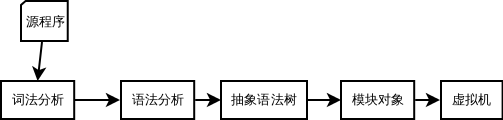
\includegraphics[scale=0.8]{file_process.png}
\label{fig:fileprocess}
\caption{解析器工作流程} 
\end{figure}


